\chapter{Results} % fixme

\section{Human3.6M}
\subsection{Evaluation protocol}
Human3.6M has 11 subjects out of which 7 are publically released while the rest are kept private. There are 2 widely used evaluation protocol. Protocol-1 is using all 4 camera views in subjects $S1$, $S5$, $S6$, $S7$ and $S8$ for training and the 
same 4 camera views in subjects $S9$ and $S11$ for validation/testing. Protocol-2 is the same as 1 expect that the predictions are post-processed via a rigid transformation
before comparing to the ground-truth.

\begin{figure}[h]
    \centering
    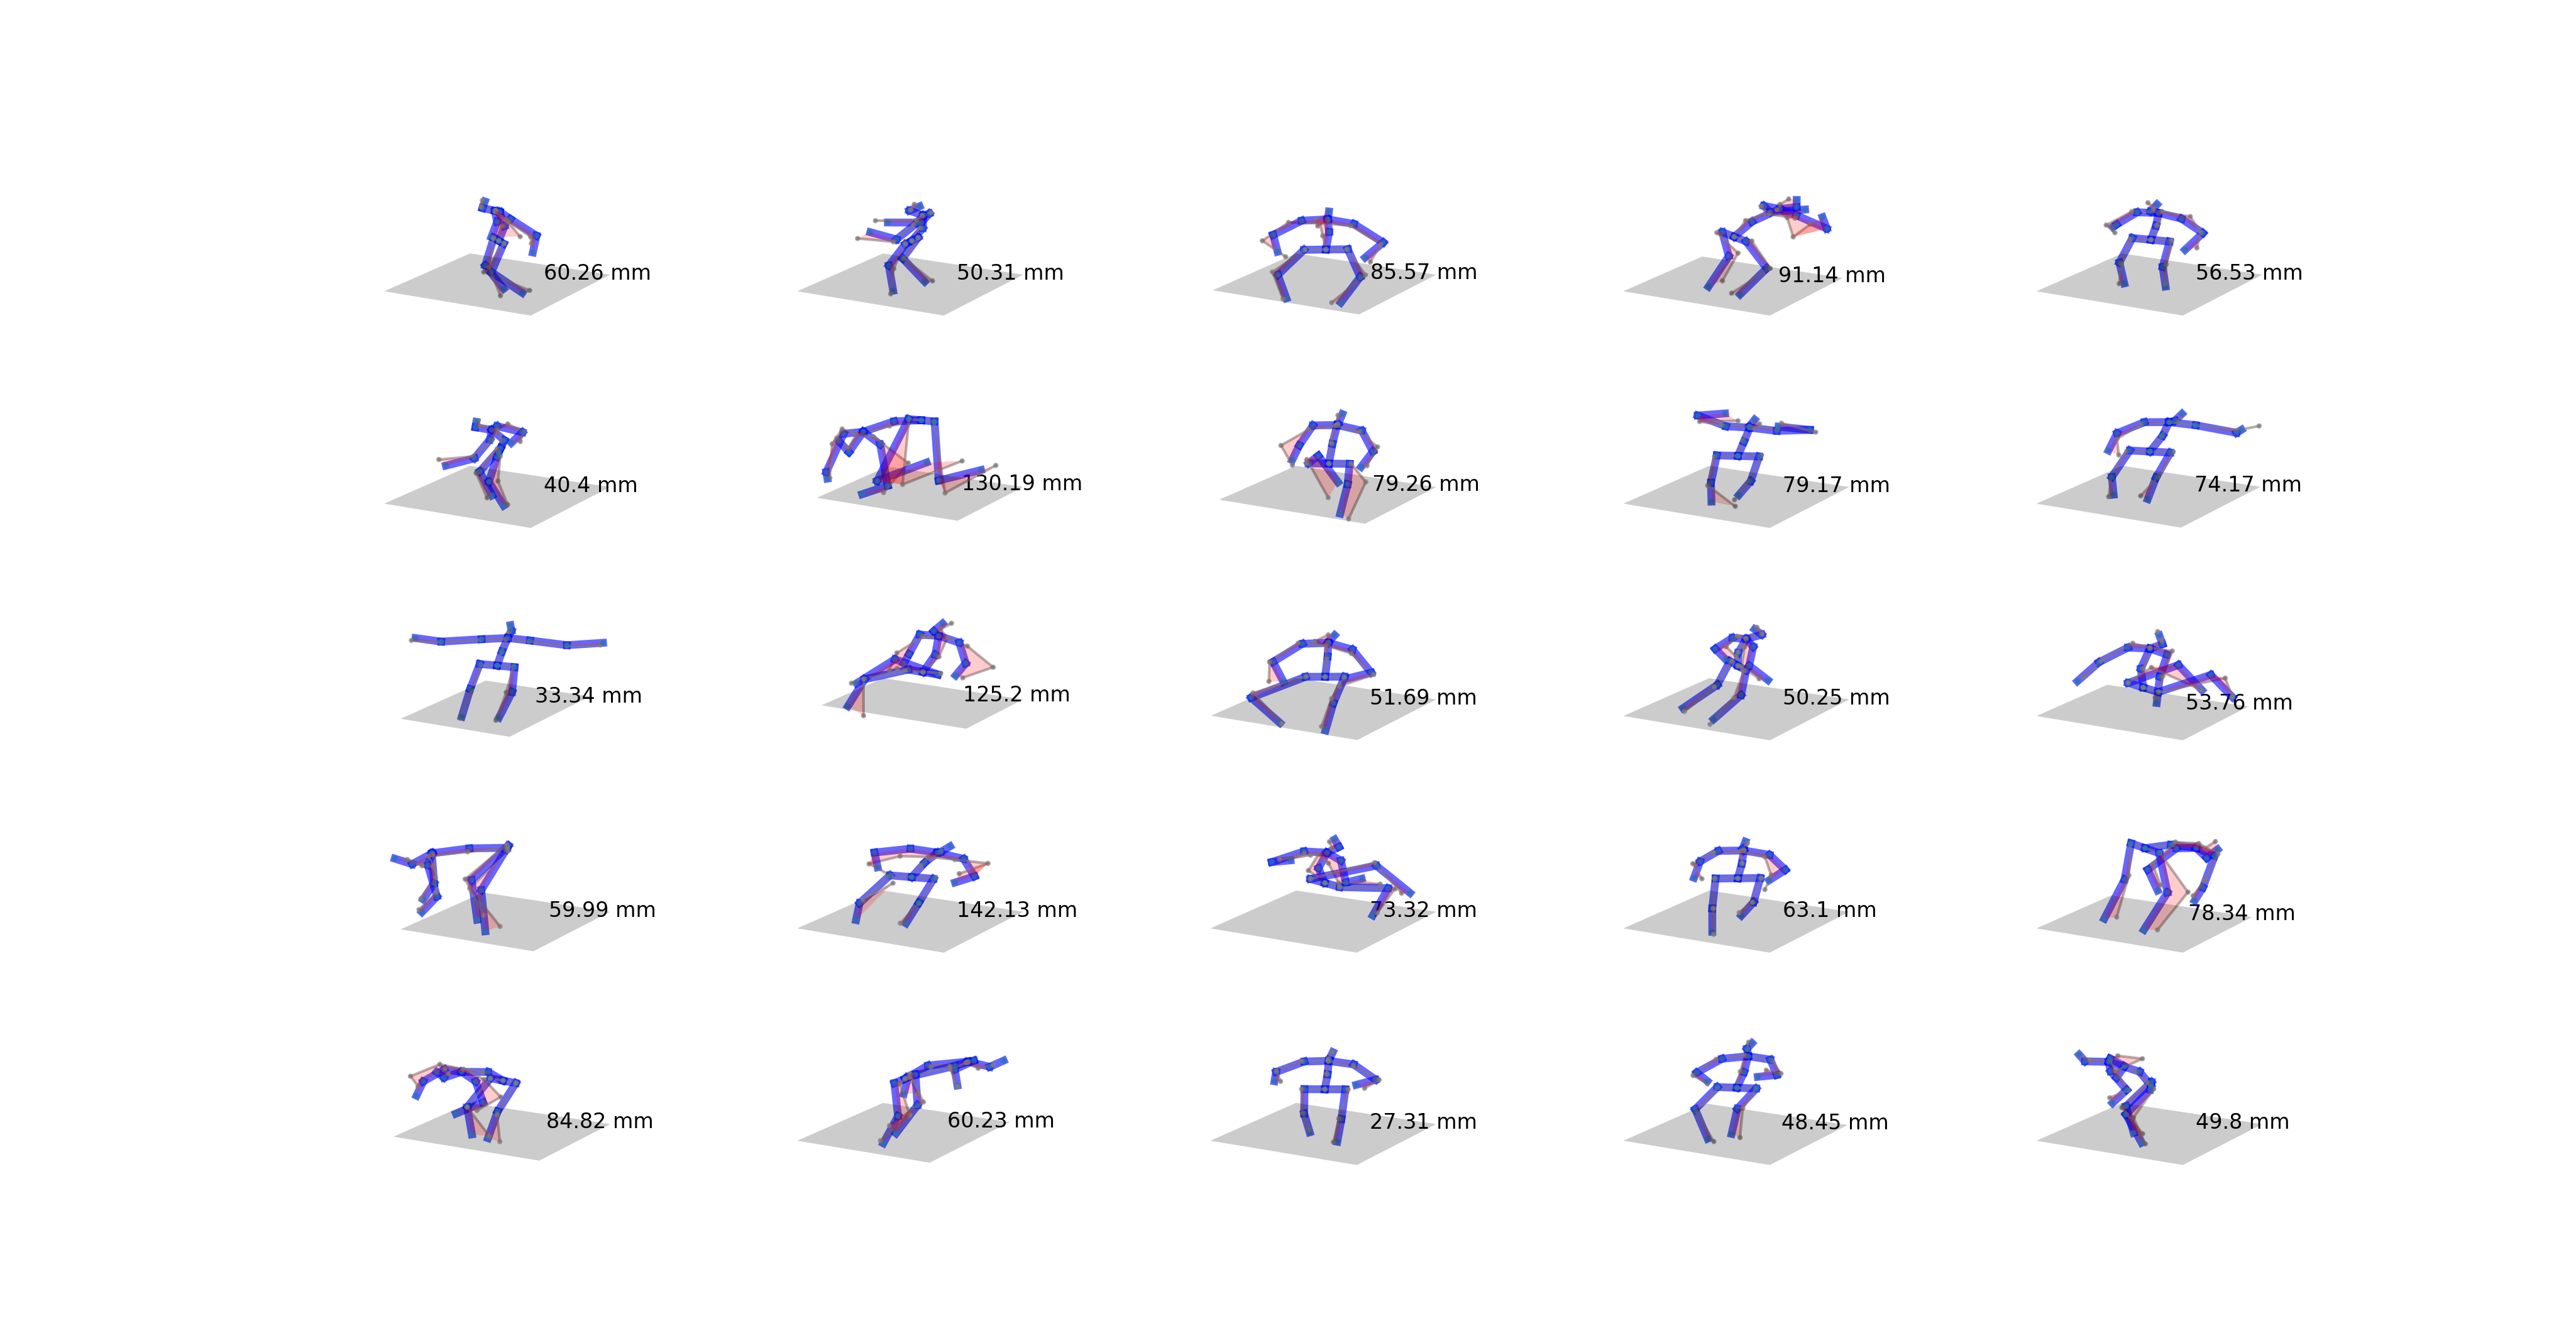
\includegraphics[width=\textwidth]{figures/results25_66mm.png}
    \caption{Comparing predictions and ground truth}
    \label{fig:results25}
\end{figure}

\subsection{2D-3D lifting}
The current experiments and results are only for 2D to 3D lifting \ac{vae} and could be found at https://app.wandb.ai/b-sridatta/hpe3d?workspace=user-b-sridatta. The results illustrated below are after training the model for 100 epochs on around 400,000 2D poses without augmentation. The architecure is as described in earlier with 512 hidden units per linear layer and 100 latent dimension and with a beta weight for \ac{kld} loss as 0.001. Further immediate experiments that have to be carried out are itegrating data augmentation, beta annealing, lower latent dimensions and image modalities. 

Figure [\ref{fig:results25}] illustrates 25 random predictions of the validation poses (in blue) and their correspsonding error (in red) w.r.t the ground truth (in gray) in millimeters. Figure[\ref{fig:latentspace}] is the visualization of 2D pose embedding in latent space after dimensionality reduction using \ac{umap} with different number of neighbours where small neighbours extract local features and large numbers extract more global features. Each action is given a unqiue color. Though we small clusters of blues, browns, pinks the overall space looks very mixed up. This is expected to be improved after annealing beta from 0 to 1 over t he course of training or by using cyclical annealing \cite{cyclicbeta}. However, it could also be the case that the many of the instance in different actions over lap. For example, the action standing up and sitting down have instances while both or standing or sitting etc. This could be verified by visualising the latent space with images rather than just points.  

\begin{figure}[h]
    \centering
    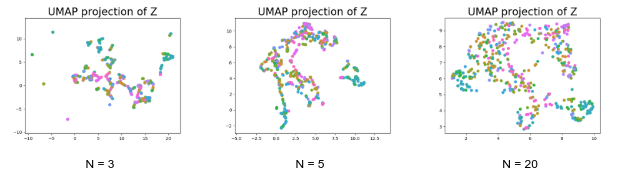
\includegraphics[width=\textwidth]{figures/latentspace.png}
    \caption{UMAP Visualization of samples in latent space with varying nearest neigbours}
    \label{fig:latentspace}
\end{figure}